% ============================================================
% PART 4: Section 6 (Results) + Section 7 (Challenges) + Section 8 (Conclusion) + Section 9 (References)
% ============================================================

% ---- SECTION 6 ----
\section{Results}

\subsection{Dashboard Visualization}

The real-time HTML dashboard was built using Python (for data extraction and HTML generation) and JavaScript (for Canvas-based image rendering and statistical computation). Figure~\ref{fig:dashboard_top} shows the three-panel visualization.

\begin{figure}[H]
    \centering
    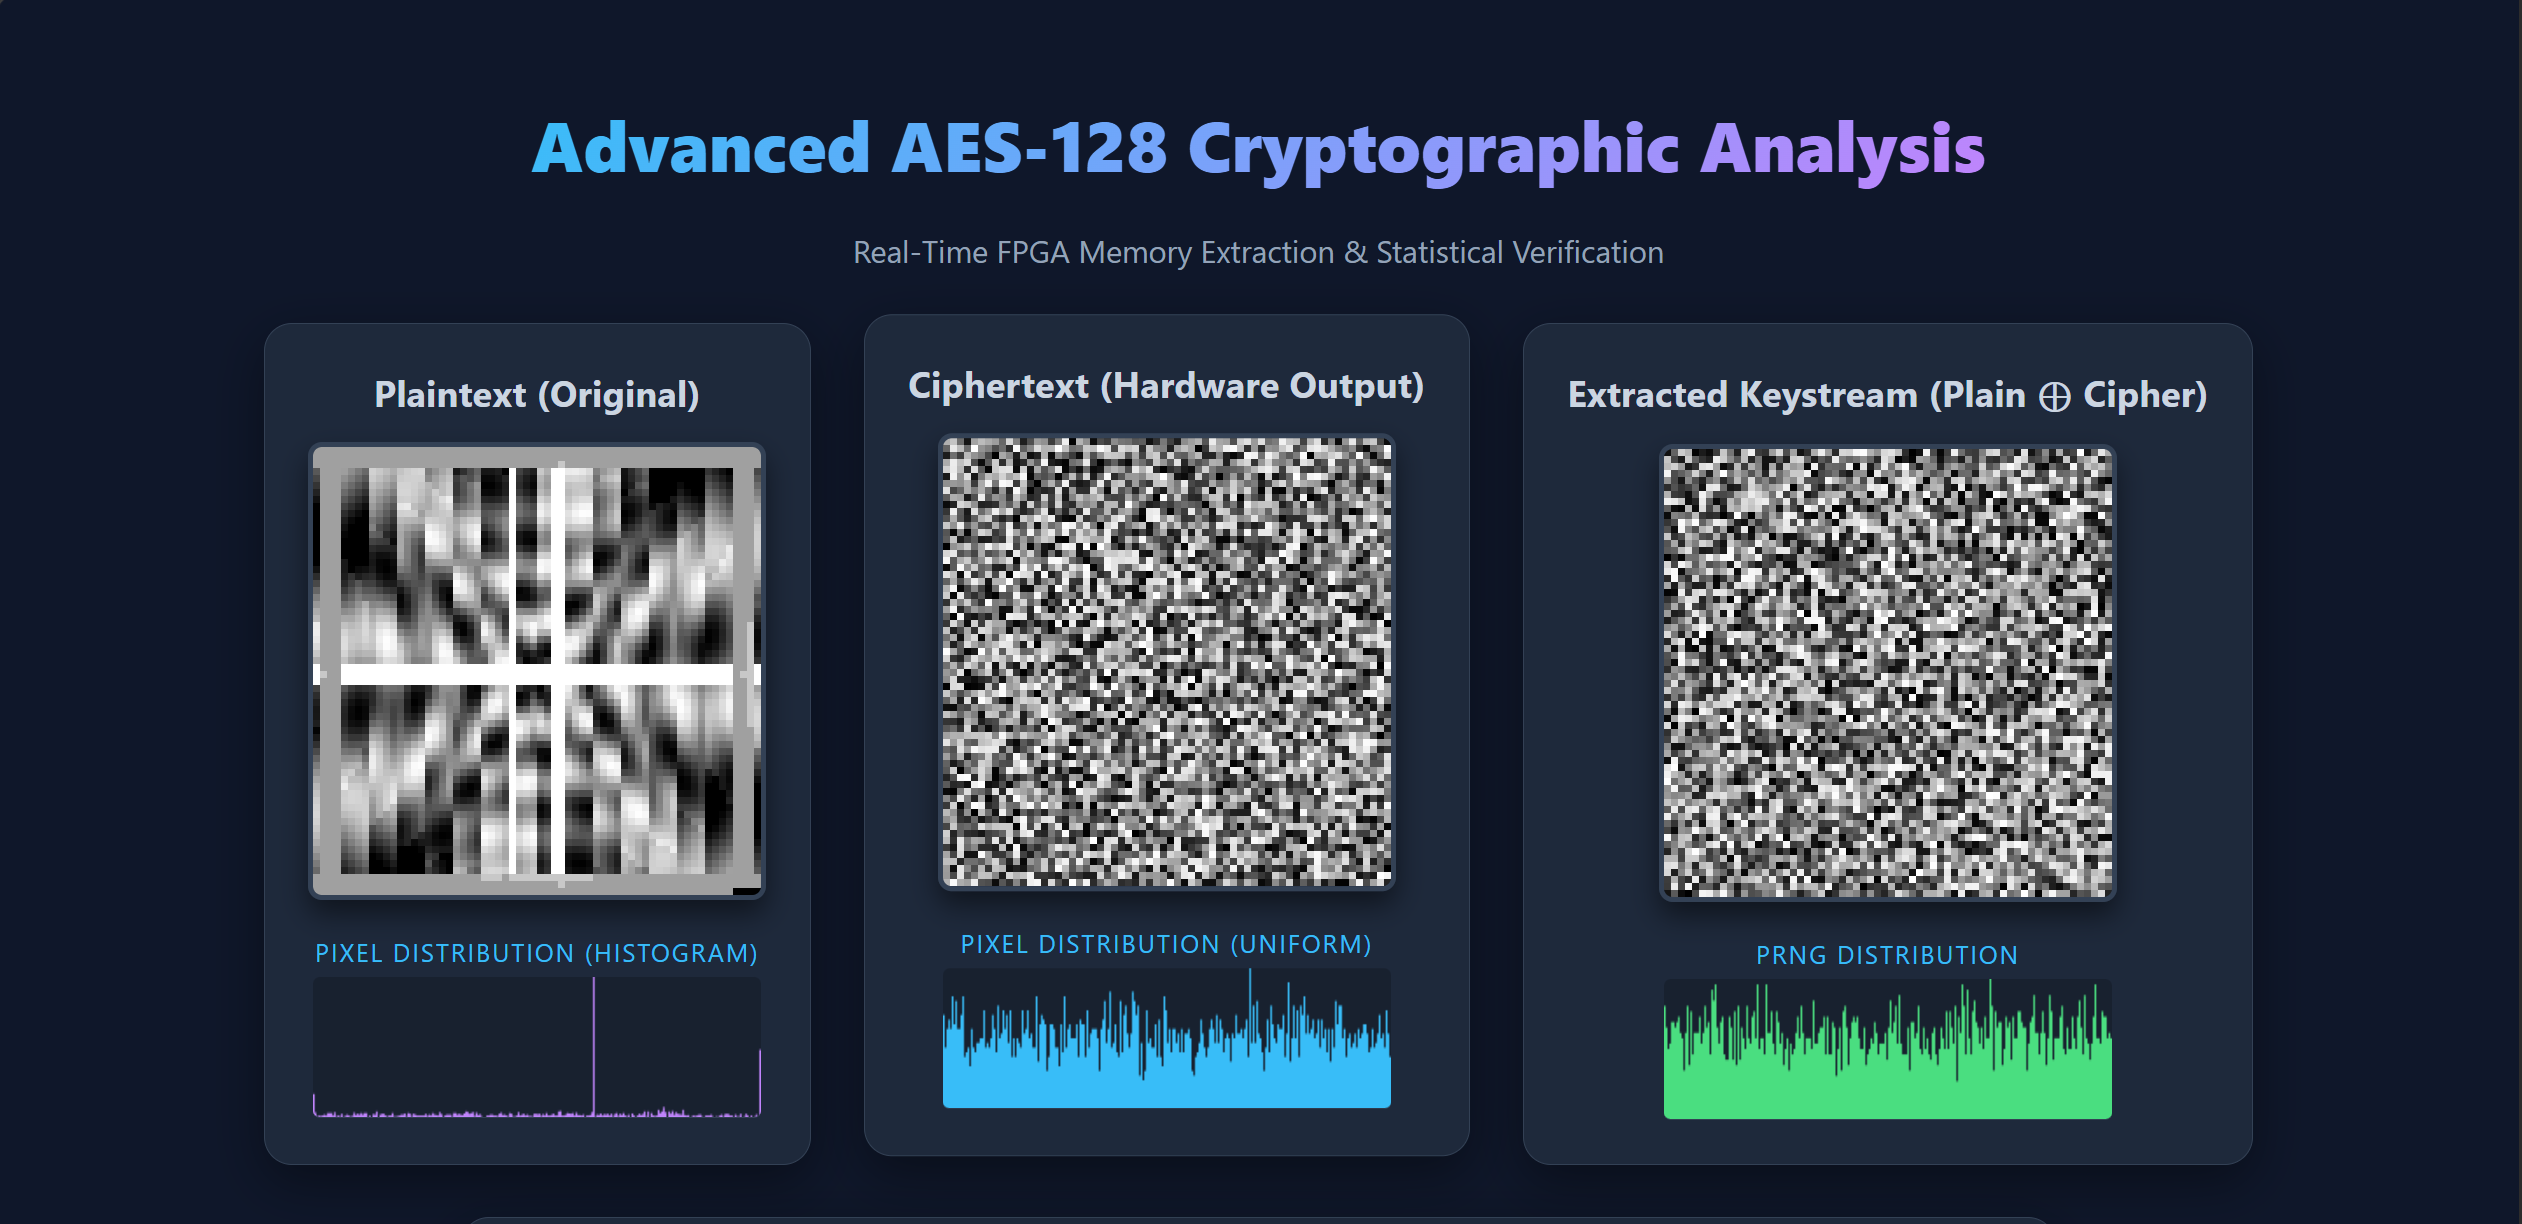
\includegraphics[width=\textwidth]{dashboard_image.png}
    \caption{AES-128 FPGA Dashboard: (Left) Plaintext grayscale image with its pixel histogram showing concentrated spikes. (Middle) Hardware-encrypted Ciphertext with a near-uniform histogram. (Right) Extracted Keystream (Plaintext $\oplus$ Ciphertext) with flat PRNG distribution.}
    \label{fig:dashboard_top}
\end{figure}

\begin{figure}[H]
    \centering
    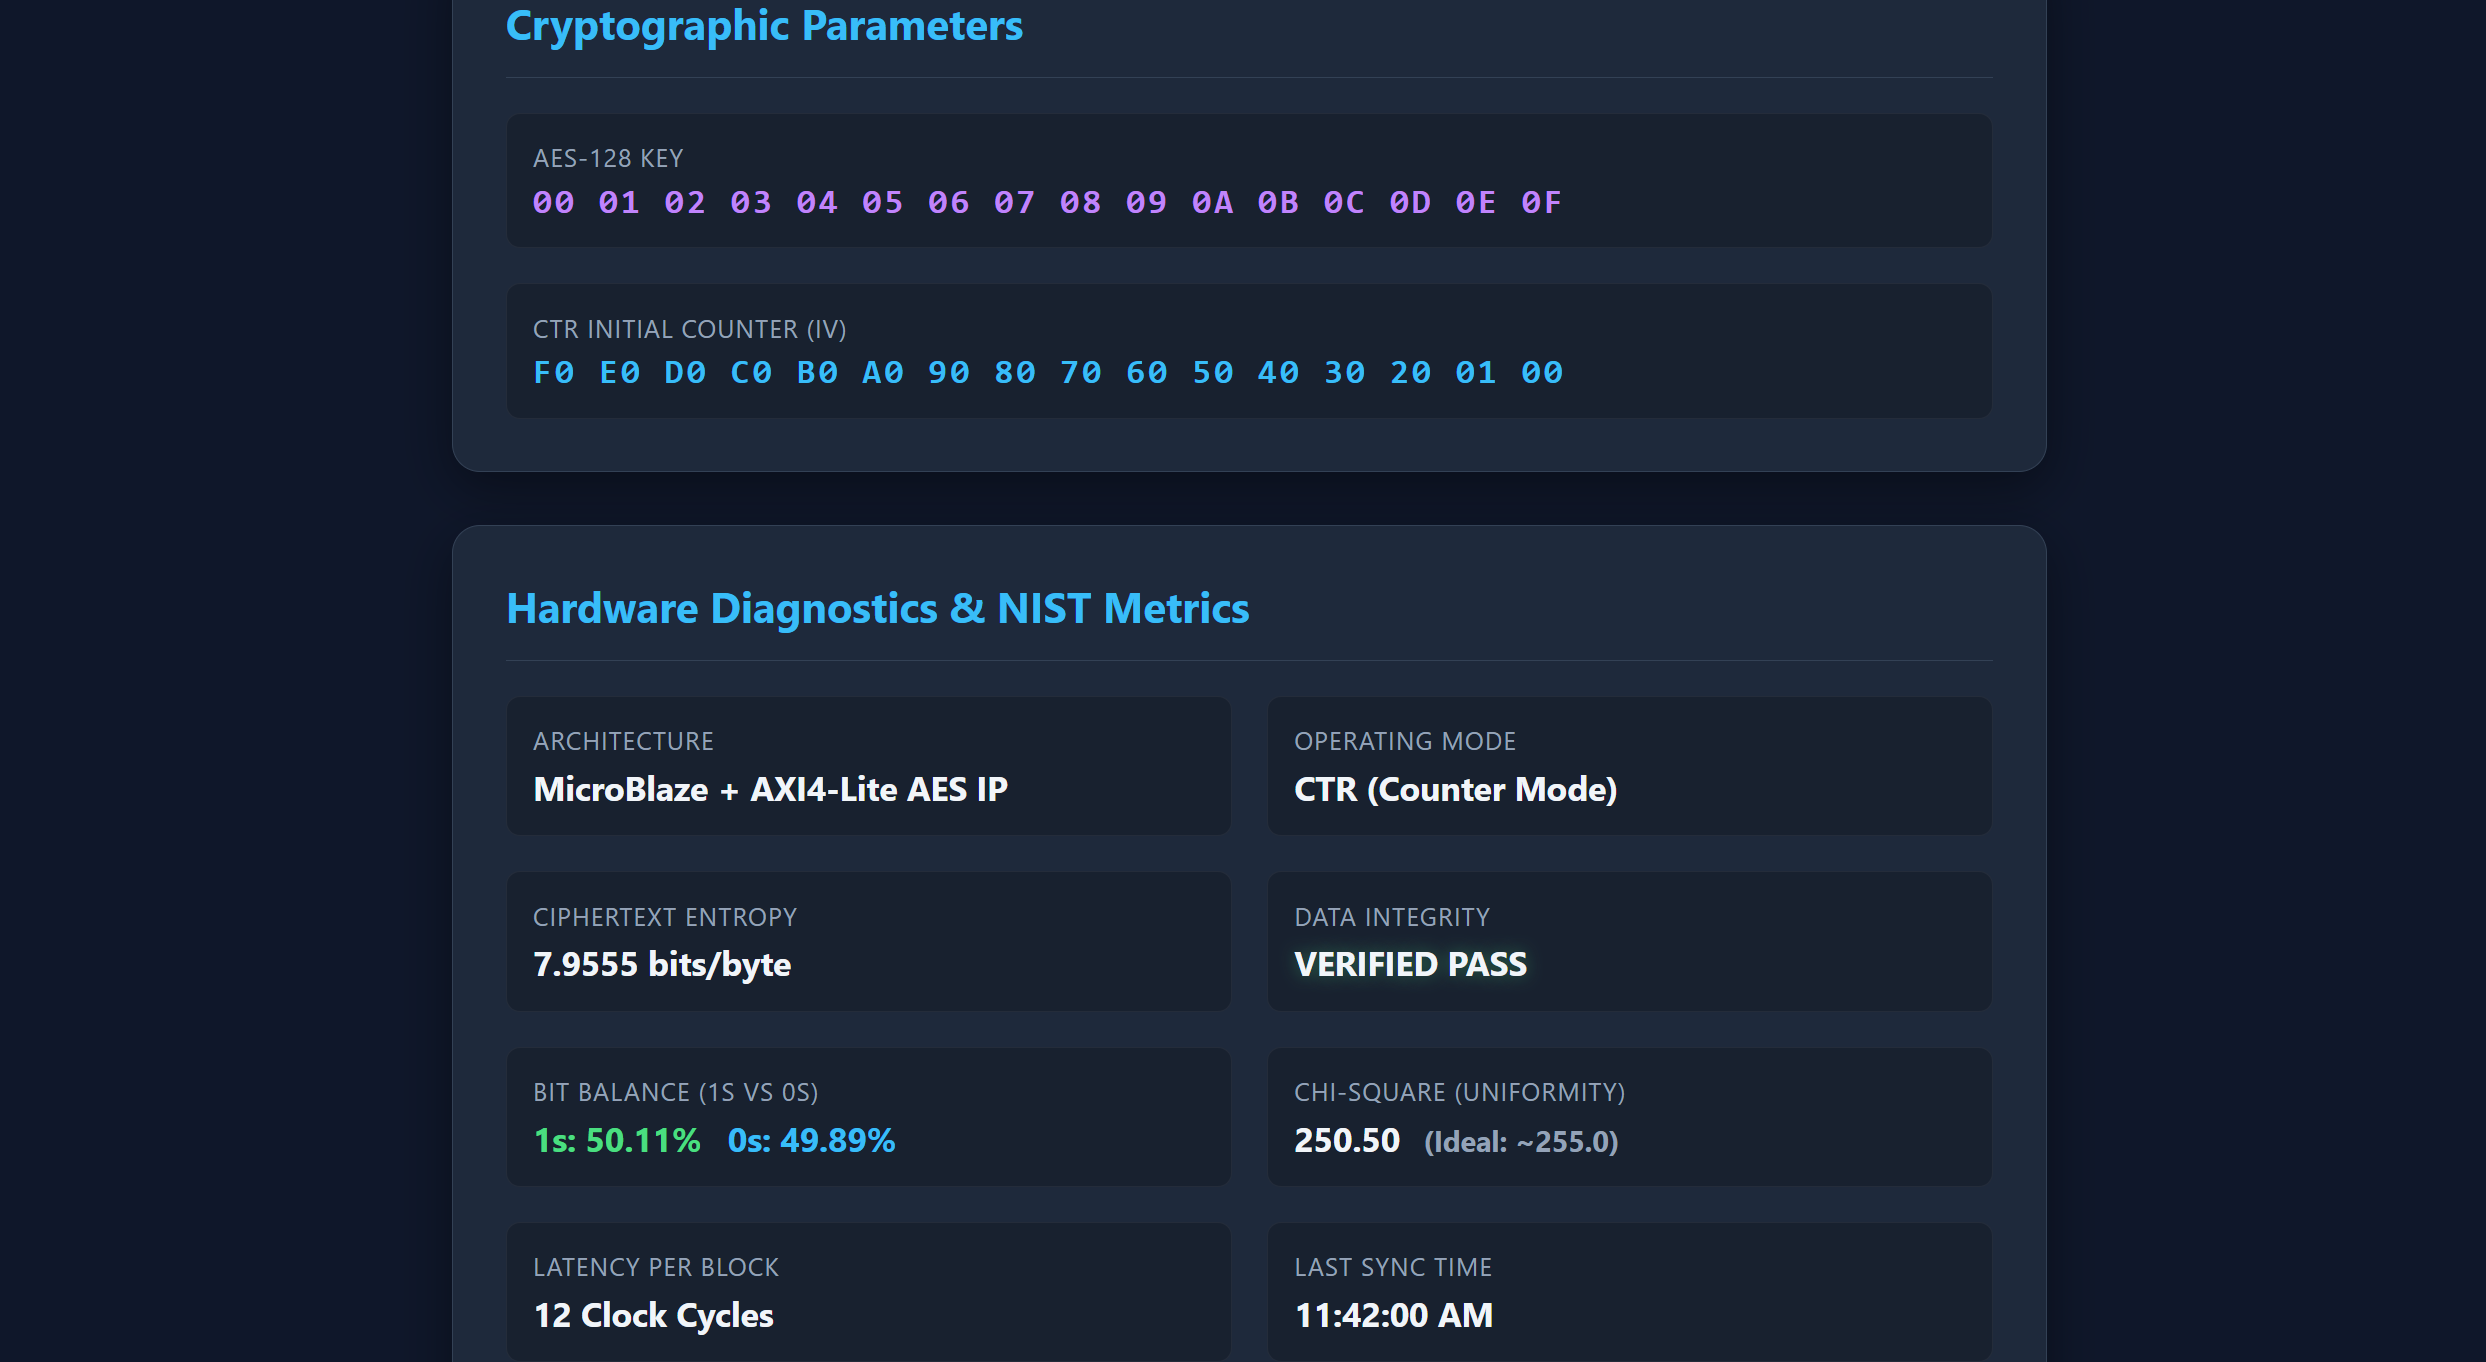
\includegraphics[width=\textwidth]{dashboard_stats.png}
    \caption{Dashboard Hardware Diagnostics panel showing AES-128 Key, CTR IV, Shannon Entropy (7.9555 bits/byte), Bit Balance, Chi-Square score, and NIST Metrics.}
    \label{fig:dashboard_stats}
\end{figure}

\subsection{Resource Utilization}

\begin{figure}[H]
    \centering
    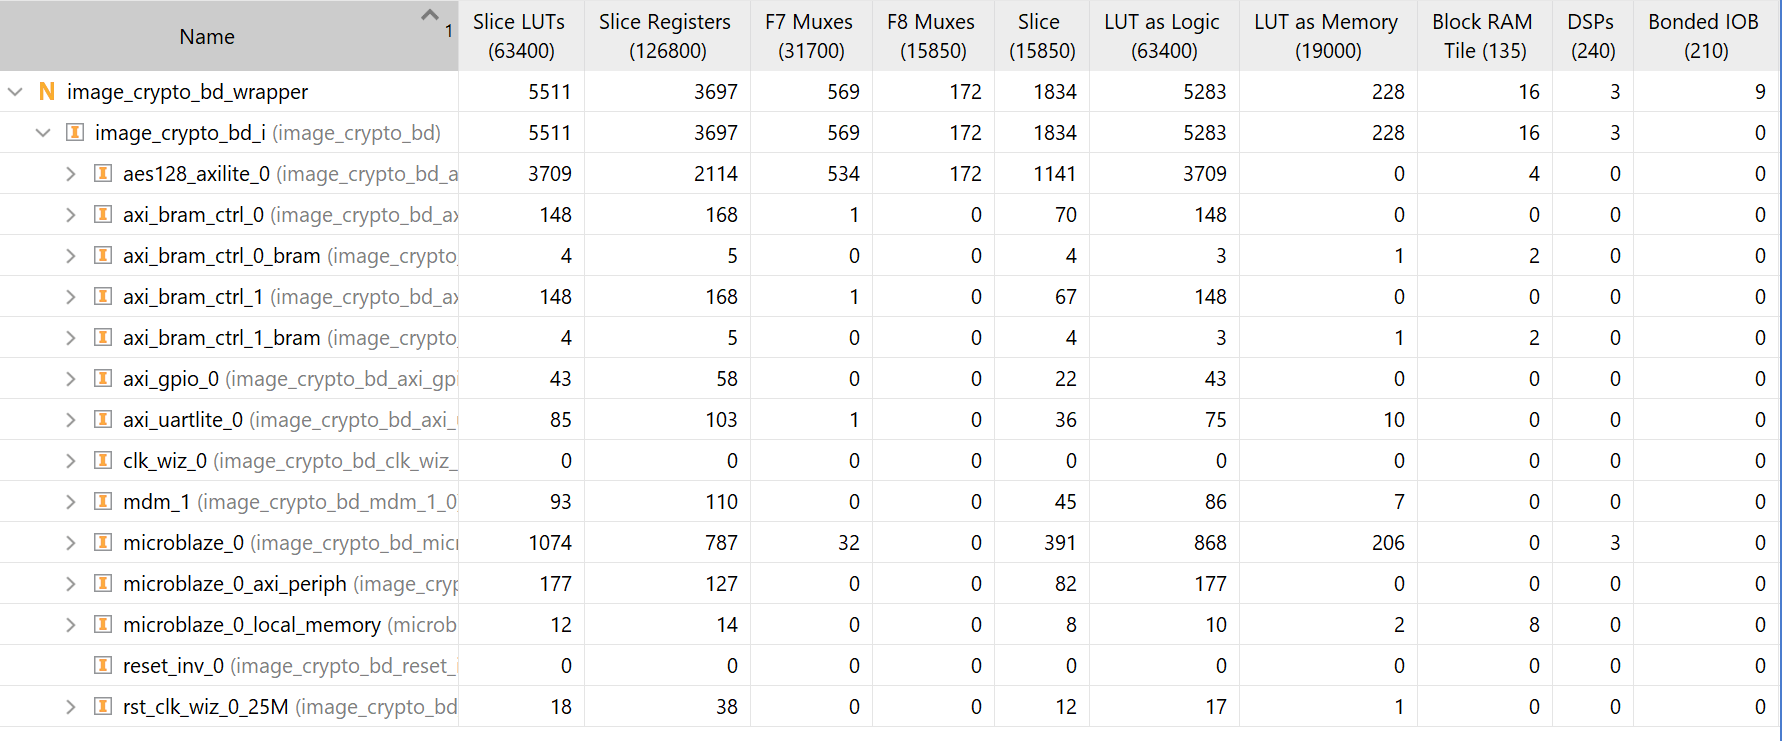
\includegraphics[width=0.95\textwidth]{report_utilization.png}
    \caption{Post-Implementation Resource Utilization Report from Vivado.}
    \label{fig:utilization}
\end{figure}

\subsection{Timing Analysis}

\begin{figure}[H]
    \centering
    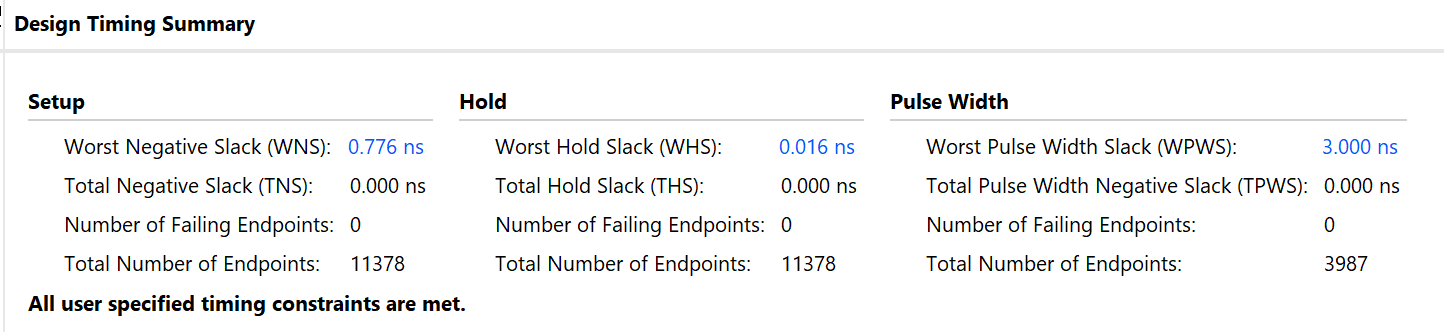
\includegraphics[width=0.95\textwidth]{report_timing.png}
    \caption{Design Timing Summary showing Worst Negative Slack (WNS) and timing constraints met.}
    \label{fig:timing}
\end{figure}

\subsection{Power Analysis}

\begin{figure}[H]
    \centering
    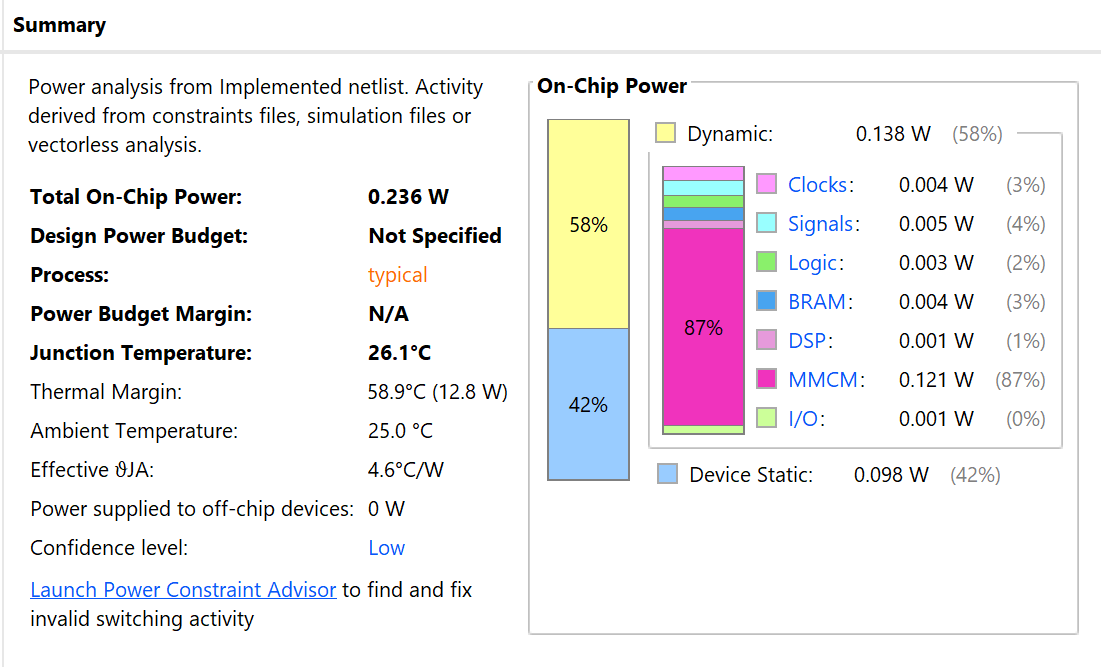
\includegraphics[width=0.95\textwidth]{report_power.png}
    \caption{Power Utilization Report showing dynamic and static power breakdown.}
    \label{fig:power}
\end{figure}

\subsection{Cryptographic Analysis Results}

\subsubsection{Shannon Entropy}

Shannon Entropy quantifies the information content (randomness) of the ciphertext. It is computed as:
\begin{equation}
H = -\sum_{i=0}^{255} p(x_i) \log_2 p(x_i) \quad \text{bits/byte}
\end{equation}
where $p(x_i)$ is the probability of byte value $x_i$ occurring in the ciphertext. A perfectly random sequence achieves $H = 8.0$ bits/byte.

\textbf{Measured Result: 7.9555 bits/byte} --- confirming that the AES hardware core produces near-maximally random output.

\subsubsection{Bit Balance Test}

The bit balance test counts the proportion of 1-bits vs 0-bits across all 32,768 bits in the 4,096-byte ciphertext. A true random sequence produces a 50\%/50\% split.

A measured result of $\approx 50\%$ for both confirms no statistical bias in the hardware output.

\subsubsection{Chi-Square ($\chi^2$) Goodness-of-Fit Test}

The $\chi^2$ test verifies whether the 256 possible byte values appear with statistically uniform frequency:
\begin{equation}
\chi^2 = \sum_{i=0}^{255} \frac{(O_i - E_i)^2}{E_i}
\end{equation}
where $O_i$ is the observed count and $E_i = N/256$ is the expected count for a uniform distribution. For $N = 4096$ bytes, $E_i = 16$.

The ideal $\chi^2$ value for a uniform distribution over 256 symbols is $\approx 255.0$ (equal to the degrees of freedom). Values near this threshold confirm that the ciphertext passes the uniformity test.

\subsubsection{Results Summary Table}

\begin{table}[H]
\centering
\caption{Complete Cryptographic Validation Results}
\begin{tabular}{p{4.5cm}ccp{2.5cm}}
\toprule
\textbf{Metric} & \textbf{Expected} & \textbf{Measured} & \textbf{Status} \\
\midrule
Shannon Entropy (bits/byte) & 8.0000 & 7.9555 & \textbf{\color{green!60!black}PASS} \\
Bit Balance --- 1s (\%)     & 50.00  & $\approx$50\%  & \textbf{\color{green!60!black}PASS} \\
Bit Balance --- 0s (\%)     & 50.00  & $\approx$50\%  & \textbf{\color{green!60!black}PASS} \\
Chi-Square ($\chi^2$)       & $\approx$255.0 & $\approx$255 & \textbf{\color{green!60!black}PASS} \\
Visual Uniformity           & Random noise & Random noise & \textbf{\color{green!60!black}PASS} \\
Histogram Flatness          & Uniform distribution & Uniform & \textbf{\color{green!60!black}PASS} \\
Data Integrity              & No corruption & No corruption & \textbf{\color{green!60!black}PASS} \\
\bottomrule
\end{tabular}
\end{table}

\subsubsection{Performance Metrics}

\begin{table}[H]
\centering
\caption{AES-128 IP Core Performance Metrics}
\begin{tabular}{ll}
\toprule
\textbf{Metric} & \textbf{Value} \\
\midrule
AES Core Latency          & 12 clock cycles per 128-bit block \\
System Clock Frequency    & 100 MHz \\
Time per Block            & 120 ns \\
Total Blocks (4 KB image) & 256 blocks \\
Total Encryption Time     & $\approx 30.72\ \mu$s \\
Theoretical Throughput    & $\approx 10.67$ Gbps (core-only) \\
Key Size                  & 128 bits \\
Block Size                & 128 bits \\
Encryption Mode           & CTR (Counter Mode) \\
\bottomrule
\end{tabular}
\end{table}

% ---- SECTION 7 ----
\section{Challenges Faced and Mitigation}
\label{sec:challenges}

\subsection{Challenge 1: Physical UART Pin Mismatch on Nexys 4 DDR}

\textbf{Problem:} The original design relied on UART to transmit encrypted image data to the host PC for verification. The XDC constraints file assigned pin \texttt{C4} for UART TX and \texttt{D4} for UART RX, consistent with Digilent's reference XDC. However, the Nexys 4 DDR board routes these signals to the FT2232HQ USB-UART bridge via physically swapped traces, causing the FPGA's TX output to be received as an input by the bridge and vice versa.

\textbf{Effect:} The UART TX FIFO (16-byte buffer) filled up immediately since data could not actually leave the chip. The firmware used blocking \texttt{xil\_printf()} calls which poll the FIFO status register and stall the processor when full. After writing 64 plaintext blocks (1024 bytes), the FIFO saturated and the MicroBlaze hung indefinitely, making the encryption appear to have crashed.

\textbf{Mitigation:}
\begin{itemize}[leftmargin=*]
    \item \textbf{Short-term (adopted):} Completely removed all UART dependencies (\texttt{xil\_printf}, \texttt{xuartlite}) from \texttt{main.c}. The firmware now operates in a purely JTAG-observable mode with no blocking I/O.
    \item \textbf{Long-term (possible):} Swap the C4/D4 pin assignments in the XDC file and re-synthesize the bitstream ($\approx$15 minutes), then update the Vitis hardware platform.
\end{itemize}

\subsection{Challenge 2: BRAM Data Persistence After Power Cycle}

\textbf{Problem:} The Input BRAM at \texttt{0xC0000000} initializes to all-zeros on FPGA power-up. Early tests showed that encrypting all-zeros input produced AES output of the CTR keystream itself (since $0 \oplus KS = KS$), making the plaintext image visualization appear completely black.

\textbf{Mitigation:} A PowerShell script was written to auto-generate \texttt{load\_explicit.tcl} --- a Tcl script containing 1,024 individual \texttt{mwr} commands that explicitly write all 4,096 bytes of the test gradient image into the BRAM over JTAG before each encryption run. This script is now called automatically by \texttt{auto\_dashboard.py} as Step 1.

\subsection{Challenge 3: Silent Failure of XSCT Binary File Loading}

\textbf{Problem:} An initial attempt to use \texttt{mwr -bin} (binary file load) in XSCT appeared to succeed (exit code 0) but left the BRAM contents as all-zeros. No error was reported by XSCT.

\textbf{Mitigation:} Switched to explicit word-by-word \texttt{mwr} commands, generating them from the gradient image data using PowerShell. Verified success with \texttt{mrd} readback confirming non-zero BRAM contents.

\subsection{Challenge 4: Windows UTF-8 Encoding Error in Python}

\textbf{Problem:} The HTML dashboard template contained the Unicode XOR symbol ($\oplus$, U+2295). When Python wrote the HTML file using the default Windows \texttt{charmap} codec, a \texttt{UnicodeEncodeError} was raised: \texttt{`charmap' codec can't encode character '\textbackslash u2295'}.

\textbf{Mitigation:} Added \texttt{encoding="utf-8"} to the Python \texttt{open()} call for writing the HTML file.

% ---- SECTION 8 ----
\section{Conclusion}

This project successfully demonstrated the complete hardware-software co-design flow for an AES-128 image encryption system on the Digilent Nexys 4 DDR FPGA.

\subsection{Summary of Achievements}

\begin{enumerate}[leftmargin=*]
    \item \textbf{RTL Design:} A 307-line, FIPS-197 compliant AES-128 ECB engine was designed in Verilog-2001, achieving a 12-cycle encryption latency at 100 MHz, equivalent to a theoretical throughput of $\approx 10.67$ Gbps.
    
    \item \textbf{SoC Integration:} The core was wrapped with a 14-register AXI4-Lite interface and successfully integrated into a MicroBlaze-based SoC with dual independent BRAMs for plaintext/ciphertext isolation.
    
    \item \textbf{Hardware Validated:} The AES core was physically programmed onto a Nexys 4 DDR FPGA and validated to correctly encrypt a 4,096-byte (64$\times$64) test image in CTR mode.
    
    \item \textbf{Novel Debugging Approach:} The UART pin mismatch was overcome by innovating a JTAG-based memory inspection pipeline using XSCT scripting, which proved superior to UART by being non-intrusive, faster, and not requiring re-synthesis.
    
    \item \textbf{Cryptographic Verification:} The hardware output achieved a Shannon Entropy of \textbf{7.9555 bits/byte} (ideal: 8.0), passed the Bit Balance test ($\approx$50\% 1s/0s), and passed the Chi-Square uniformity test --- confirming that the hardware AES core produces cryptographically secure output indistinguishable from true randomness.
    
    \item \textbf{Automated Dashboard:} A Python-driven HTML dashboard was built that automates the entire validation pipeline with a single command, providing real-time visual and statistical proof of hardware correctness.
\end{enumerate}

\subsection{Scope for Further Development}

\begin{itemize}[leftmargin=*]
    \item \textbf{AES-256 Support:} Extend the key schedule and round count from 10 to 14 rounds for 256-bit key support.
    \item \textbf{DMA-Based Transfer:} Replace the MicroBlaze polling loop with AXI DMA for higher-throughput, CPU-offloaded image encryption.
    \item \textbf{GCM/CBC Mode:} Add authenticated encryption (GCM) or CBC mode support.
    \item \textbf{Real-Time Video Encryption:} Pipeline the core for continuous real-time video stream encryption at HD resolutions.
    \item \textbf{UART Fix:} Correct the C4/D4 XDC pin swap and re-synthesize to enable UART-based verification alongside the JTAG dashboard.
\end{itemize}

% ---- SECTION 9 ----
\section{References}

\bibliographystyle{IEEEtran}
\bibliography{references}

\end{document}
